\documentclass[a4paper, openany]{book}
\usepackage[T1]{fontenc}%per rappresentare i font italiani, come le lettere accentate, con la giusta spaziatura
\usepackage[utf8]{inputenc}%per poter inserire nel testo .tex i caratteri unicode8
\usepackage[italian]{babel}%per poter effettuare la giusta sillabazione della lingua italiana
\usepackage{classicthesis}%necessario per usare lo stile arsclassica
\usepackage{arsclassica}%per poter usare lo stile arsclassica usato nell'Arte di imparare il Latex
\usepackage{amsmath}%per poter rappresentare ed utilizzare al meglio gli ambienti e le formule matematiche
\usepackage{amssymb}%per rappresentare alcuni simboli particolari matematici
\usepackage{amsthm}%per definire e poter effettuare le dimostrazioni matematiche
\usepackage{amsfonts}%per poter avere i font matematici
\usepackage{amstext}%per avere una gestione del testo nell'ambiente matematico
\usepackage{booktabs}%per la corretta gestione delle tabelle
\usepackage{microtype}%per effettuare un aggiustamento della spaziatura tra caratteri e del font
\usepackage{clrscode3e}%per effettuare lo pseudocodice nello stile del libro CLRS
\usepackage{graphicx}

\theoremstyle{definition}%per avere lo stile tondo quando uso un ambiente definito da newtheorem
\newtheorem*{defi}{Def}%Definizione per avere la gestione delle definizioni
\newtheorem{prop}{Prop}[chapter]
\newtheorem{thm}{Thm}[chapter]
\newtheorem{esempio}{Esempio}
\newcommand{\numberset}{\mathbb}
\newcommand{\N}{\numberset{N}}
\newcommand{\deriv}{\Rightarrow}

\begin{document}
    \title{Data Mining notes}
    \author{Marco Natali}
    \date{}
    \maketitle

    \tableofcontents
    \listoffigures

    \chapter{Introduction}
This course will provide an introduction to AI techniques and approach analyzed nowadays and to understand
the current state of art we have to provide an Timeline to see progress and discover done during the time,
so in figure \ref{img:timeline} we will see all important events related with AI.

\begin{figure}
    \caption{AI Timeline evolution}
    \label{img:timeline}
    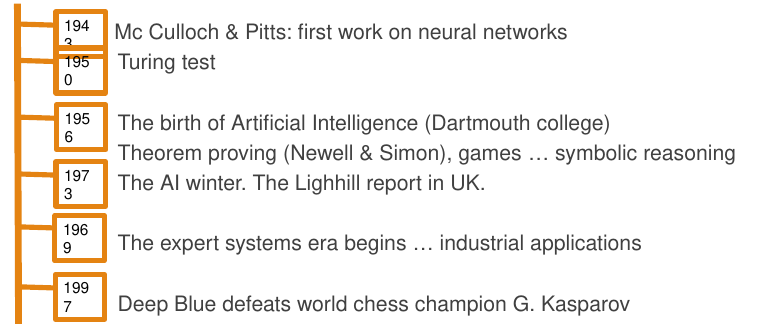
\includegraphics[width=\textwidth]{Images/timeline}
    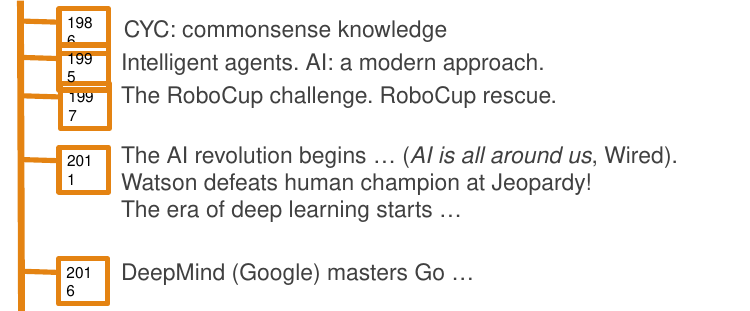
\includegraphics[width=\textwidth]{Images/timeline2}
\end{figure}
The major discover happened on $2020$ are the following:
\begin{description}
    \item [GPT3 (Generative Pre-trained Transformer): ] produced by OpenAI in May $2020$, is 
           a larger and richer language model consisting in $175$ billion machine learning parameters
           used for automatic text generation, translation, user interface synthesis
    \item [DARPA challenge (AlphaDogFights)] with simulated F-16 Air Fighters where on $18-20$ August $2020$
           there was the final Event, where AI system was against each other and the winner was a system by 
           Heron system, that was also able to defeated a human expert top gun fighter $5-0$.
\end{description}
On \cite{andrewNg} Andrew NG says that AI will transform many industries, but it’s not magic and 
almost all of AI’s recent progress is based on one type of AI, in which some input data $(A)$ is used to
quickly generate some simple response $(B)$ [$A \to B$].\newline
Also Andrew Ng says that if a typical person can do a mental task with less than one second of thought,
we can probably automate it using AI either now or in the near future.\newline
Choosing A and B creatively has already revolutionized many industries, it is poised to
revolutionize many more.

ML systems are not (yet?) able to justify in human terms their results, so for some application it is essential
the human knowledge to be able to generate explanations, infact some regulations requires the right
to an explanation in decision-making, and seek to prevent discrimination based on race, opinions,
health, sex and so on, like GPDR.\newline
ML systems learn what’s in the data, without understanding what's true or false, real or imaginary, 
fair or unfair and so it is possible to develop bad/unfair models.

The goal of building AI systems is far from being solved and is still quite challenging in its own.
Building complex AI systems requires the combination of several techniques and approaches, not only ML.\newline
One of the most challenging tasks ahead of us is integration of
perception and reasoning in AI systems.

AI fundamentals is mostly about “Slow thinking” or “Reasoning” and AI fundamentals has the role,
within the AI curriculum, of teaching you about the foundations of a discipline which is now 60 year old.\newline
We will cover different approaches, also some coming of the “Good Old-
Fashioned Artificial Intelligence” (GOFAI) or symbolic AI.

\begin{defi}
Symbolic AI is an high-level "symbolic" (human-readable) representations of problems, the 
general paradigm of searching for a solution, knowledge representation and reasoning, planning.\newline
Symbolic AI was the dominant paradigm of AI research from the mid 1950s until the late 1980s and 
central to the building of AI systems is the \emph{Physical symbol systems hypothesis}, formulated by Newell and Simon.
\end{defi}

The approach is based on the assumption that many aspects of intelligence can be achieved by the 
manipulation of symbols (the physical symbol system hypothesis):
\begin{defi}
A physical symbol system has the necessary and sufficient means for general intelligent action
\end{defi}%CITE WHO SAYS THAT
Human thinking is a kind of symbol manipulation system (a symbol system is necessary for intelligence) and 
machines can be intelligent (a symbol system is sufficient for intelligence).\newline
The hypothesis cannot be proven, we can only collect empirical evidence and observations and experiments
on human behavior in tasks requiring intelligence.

We have two different typologies of AI, that was introduced and considered:
\begin{description}
    \item [Strong AI: ] relies on the strong assumption that human intelligence can be reproduced
                        in all its aspects (general A.I.).\newline
                        It includes adaptivity, learning, consciousness and not only pre-programmed behavior.
    \item [Weak AI: ]   simulation of human-like behavior, without effective thinking/understanding and 
                        no claim that it works like human mind; it is the dominant approach today.
\end{description}
A problem of AI is that computer can't have needs, cravings or desires and Abraham Maslow's define 
a hierarchy of human needs:
\begin{enumerate}
    \item Biological needs (food, sleep, sex, ...)
    \item Safety, protection from environment
    \item Love and belonging, friendship
    \item Self esteem and respect from others
    \item Self-actualization
\end{enumerate}
%Introduction Chapter
    \chapter{Data Visualization}
For preparing data for data mining task it is essential to have an overall picture of your data, so we have to
gain insight in your data, with respect to your project goals and should be general to understand properties.\newline
You should discover semantics of data and also to discover statistical charecteristics of your data in
order to have a more understanding of data.

Data can be represent usually by $3$ modes:
\begin{itemize}
    \item Record: we have a matrix representation that will represent data and it is divided in:
            \begin{itemize}
                \item Data Matrix: If data objects have the same fixed set of numeric attributes,
                      then the data objects can be thought of as points in a multidimensional space,
                      where each dimension represents a distinct attribute.\newline
                      Such data set can be represented by an $m$ by $n$ matrix, where there are $m$ rows,
                      one for each object, and $n$ columns, one for each attribute,
                      as you can see in figure \ref{img:dataMatrix}.
                \item Document Matrix: each document becomes a ‘term’ vector, where each term 
                      is a component (attribute) of the vector and the value of each component is 
                      the number of times the corresponding term occurs in the document.
                \item Transition Data: A special type of record data, where each record (transaction)
                      involves a set of items, so for example consider a grocery store.\newline
                      The set of products purchased by a customer during one shopping trip constitute a transaction,
                      while the individual products that were purchased are the items,
                      as it possible to note in figure \ref{img:transiction}.
            \end{itemize}
    \item Graph
    \item Order
\end{itemize}
Data is a collection of data objects and their attributes, where the last one is a property or 
characteristic of an object like eye color of a person and a data object is a collection of 
attributes that descrive an object.

There are different types of attributes:
\begin{description}
    \item [Nominal/Categorical: ] attribute values in a finite domain, categories, “name of things” like
                                  eye color, zip codes.
    \item [Binary: ] nominal attribute with only $2$ states ($0$ and $1$) where we have \emph{symmetric binary},
                     in which both outcomes are equally important, or also \emph{asymmetric binary} where 
                     outcomes are not equally important, like medical test positive vs negative, and the convention
                     is to assign $1$ to most important outcome.
    \item [Ordinal: ] finite domain with a meangniful ordering on the domain, like rankings, grades and height.
    \item [Numeric: ] quantity (integer or real-valued) measured on a scale of equal-sized units and which
                      values have order, example of this data are temperatures in Celsius and calendar dates.
    \item [Ratio-scaled: ] we can speak of values as being an order of magnitude larger than the unit of measurement
                           and example are length, elapsed time and so on.
\end{description}
There is also a distinction about which data an attribute can have:
\begin{description}
    \item [Discrete Attribute: ] has only a finite or countably infinite set of values and often are represented
                                 as integer variables, where we can note that binary attributes are a special
                                 case of discrete attributes.
    \item [Continuous Attribute: ] has real numbers as attribute values and practically real values can only
                                   be measured and represented using a finite number of digits.\newline
                                   Examples are temperature, weight, or height and also continuous attributes
                                   are typically represented as floating-point variables.
\end{description}
The type of an attribute depends on which of the following properties/operations it possesses:
\begin{description}
    \item [Distinctness: ] $= \neq$
    \item [Order: ] $< >$
    \item [Differences: ] are $+ -$
    \item [Ratios: ] are $* /$
\end{description}
We have that Nominal attribute has only distinctness, ordinal attribute add the order property, interval
attribute has also differences and in the end ratio attribute has all $4$ properties.

Poor data quality negatively affects many data processing efforts infact we have that the most important point
is that poor data quality is an unfolding disaster and also poor data quality costs to a typical company
at least $10\%$ of revenue, but $20\%$ is probably a better estimate.

Some \emph{Data quality} issues are the following:
\begin{description}
    \item [Syntactic accuracy: ] entry is not in the domain, like write "fmale" in gender, and that can be 
                                  checked and solve quite easy.
    \item [Semantic accuracy: ] entry is in the domain but not correct, like "Bergamo is in France", and 
                                that type of error needs more information to be checked ("business rules").
    \item [Completeness: ] is violated if an entry is not correct although it belongs to the domain of the attribute,
                           and that happens when complete records are missing so the data is biased.

    \item [Unbalanced data: ] the data set might be biased extremely to one type of records.
    \item [Timeliness: ] is the available data up to date?
\end{description}
Data set may include data objects that are duplicates, or almost duplicates of one another and that is 
a major issue when we are merging data from heterogeneous sources, an example can be a same person with
multiple email addresses.
\emph{Data cleaning} is the process of dealing with duplicate data issues and consists to discover 
missing data and outlier with the purpose to remove all or at least a largest part.

In figure \ref{img:rescale} we can see that in $2001$ there was the change from Lira to Euro and 
that explain a dramatic reduction on a problem so we have to rescale values that makes consistent data.

The distribution of data observation is important to recognize if we have symmetric data, skewed data, bimodal
pattern (which usually shows subpopulation on attribute) and when visualisations reveal patterns or exceptions,
then there is “something” in the data set; when visualisations do not indicate anything specific,
there might still be patterns or structures in the data that cannot be revealed by the corresponding
(simple) visualisation techniques.


We will define now what we intend when we talk about outlier:
\begin{defi}
    Outliers are data objects with characteristics that are considerably different than most of the other
    data objects in the data set.
\end{defi}
There are two different cases: one when Outliers are noise that interferes with data analysis and another
when Outliers are the goal of our analysis, like in credit card fraud and intrusion detection.\newline
Outliers cause data quality problems and should be exceptional or an unusual data objects, so 
outliers coming from erroneous data should be excluded from the analysis and even if the outliers are correct
(exceptional data), it is sometime useful to exclude them from the analysis.\newline
For example, a single extremely large outlier can lead to completely misleading values for the mean value.

To detect an outlier we can do the following actions:
\begin{description}
    \item [Single Attribute: ] when we have an outlier in categorial attributes we can find it when we have 
                               a value that occurs with an extremely lower frequency than other; in case we 
                               want to discover an outlier in numerical attributes we use box plots.
    \item [Multidimensional Attribute: ] we can use Scatter plots for visually detect outliers for two attributes or
                                         also we can use PCA or MDS plots to discover outliers.
\end{description}
For some instances values of single attributes might be missing, due to a missing a collection of an information,
broken sensors and also attributes may not be applicable to all cases, and also missing value might not
necessarily be indicated as missing, we can use instead zero or default values.

\section{Data Preparation}
Data preparation uses informations from data understanding to select attributes, reduce the data dimension,
select records, treat missing values, treat outliers, integrate, unify and transform data 
and in the end we can improve data quality.

In Data Preparation can be execute the following operations:
\begin{description}
    \item [Aggregation: ] combining two or more attributes (or objects) into a single attribute (or object)
                          with the purpose of reduce the number of attributes/objects, have more stable
                          data and also to change the scale, like aggregate cities into regions.\newline
                          In figure \ref{img:stableData} it is possible that aggregation from number of precipitation
                          from a month in Australia in number of precipitation in a year make more stable data.
                          \begin{figure}
                            
                              \label{img:stableData}
                          \end{figure}
    \item [Data Reduction: ] we reduce the amount of data that can be done in two ways:
                             \begin{itemize}
                                \item Reduce the number of records, using Data Sampling and Clustering.
                                \item Reduce the number of columns (attributes), where we select a subset
                                      of attributes and we generate a new (a smaller) set of attributes
                             \end{itemize}
                             \emph{Sampling} is the main technique employed for data reduction and it
                             is often used for both the preliminary investigation of the data 
                             and the final data analysis.\newline
                             Sampling is typically used in data mining because processing the entire set of data
                             of interest is too expensive or time consuming.

                             The key principle for effective sampling is to using a sample that will work
                             almost as well as using the entire dataset, if the sample is \emph{representative},
                             that happens if the same has approximately the same properties as 
                             the original set of data.
                            
                             The types of Samplings are the following:
                             \begin{description}
                                 \item [Simple Random Sampling: ] there is an equal probability of selecting
                                        any particular item and we can have sampling without and with replacement.
                                 \item [Stratified Sampling: ] split the data into several partitions and 
                                        then draw random samples from each partition and we create an
                                        approximation of the percentage of each class; it is suitable 
                                        for distribution with peaks, in which each peak is a layer.
                             \end{description}
    \item [Dimension Reduction: ] selection of a subset of attributes that is as small as possible
                                  and sufficient for the data analysis.\newline
                                  Consist in removing (more or less) irrelevant features, that contain no 
                                  information useful for data mining (students ID is irrelevant in predicting 
                                  student GPA), and also removing redundant features, that duplicate much or 
                                  all of the information contained in one or more other attributes.\newline
                                  When dimensionality increases, data becomes increasingly sparse in the
                                  space that it occupies(curse of dimensionality) and also definitions of
                                  density and distance between points, which are critical for clustering
                                  and outlier detection, become less meaningful.

                                  The reduction of dimension has the purpose to avoid curse of dimensionality,
                                  reduce amount of time and memory required by datamining algorithms, 
                                  allow data to be more easily visualized and 
                                  may help to eliminate irrelevant features or reduce noise.

                                  It uses PCA(Principal Components Analysis), Singular Value Decomposition
                                  or other supervised and non-linear techniques.
                                
                                  For removing irrelevant features, a performance measure is needed that
                                  indicates how well a feature or subset of features performs and for removing
                                  redundant features, either a performance measure for subsets of features or a
                                  correlation measure is needed.

                                  To reduce the dimension we usually use these $3$ methods:
                                  \begin{description}
                                      \item [Filter Method: ] selection after analyzing the significance and 
                                                              correlation with other attributes (preprocessing)
                                      \item [Wrapper Method: ] selecting the top-ranked features using 
                                                               as reference a DM task and there is an incremental
                                                               selection of the “best” attributes, with respect
                                                               of information gain.
                                      \item [Embedded Method: ] selection as part of the data mining algorithm,
                                                                so during the operation of the DM algorithm,
                                                                the algorithm itself decides which attributes to use
                                                                and which to ignore, like Decision tree.
                                  \end{description}
    \item [Feature Creation: ] create new attributes that can capture the important information in a dataset
                               much more efficiently than the original attributes and 
                               there are two general methodologies:
                               \begin{itemize}
                                   \item Feature construction: in figure \ref{img:featureCreation} can be seen
                                         an example on how to create a new feature.
                                   \item Feature projection: it transforms the data in the high-dimensional space
                                         to a space of fewer dimensions and this transformation may be linear,
                                         or nonlinear.\newline
                                         It uses
                               \end{itemize}

                               \begin{figure}
                                    \caption{Example of Feature Creation}
                                    \label{img:featureCreation}
                                    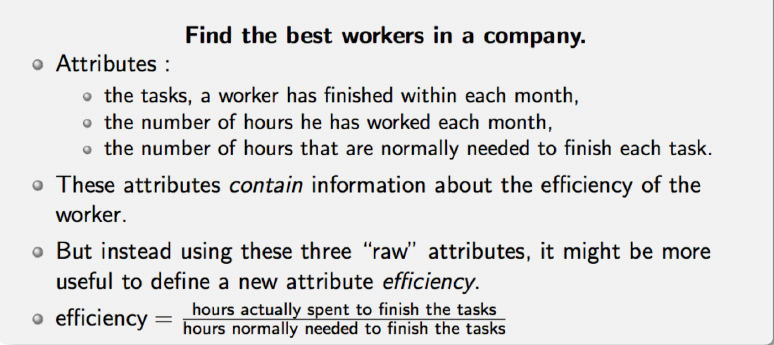
\includegraphics[width=\textwidth]{Images/featureCreation}
                               \end{figure}
The data transformation may be linear, or nonlinear.
Approaches:
–
 Principal Component Analysis (PCA)
–
 Singular Value Decomposition (SVD)
–
 Non-negative matrix factorization (NMF)
–
 Linear Discriminant Analysis (LDA)
–
 Autoencoder


\end{description}
Data Cleaning
• How to handle anomalous values
• How to handle outliers
• Data Transformations

Manage Missing Values
1.
2.
EliminaRon of records
SubsRtuRon of values
Note: it can influence the original distribu7on of numerical values
–
 Use mean/median/mode
–
 Es7mate missing values using the probability distribu7on of
exis7ng values
–
 Data Segmenta7on and using mean/mode/median of each
segment
–
 Data Segmenta7on and using the probability distribu7on within
the segment
–
 Build a model of classifica7on/regression for compu7ng missing
values

Discretization is the process of converting a
continuous attribute into an ordinal attribute
– A potentially infinite number of values are mapped into a
small number of categories
– Discretization is commonly used in classification
– Many classification algorithms work best if both the
independent and dependent variables have only a few
values

Hard to understand the optimal discretization
– We should need the real data distribution
• Original values can be continuous and sparse
• Discretized data can be simple to be interpreted
• Data distribution after discretization can have a Normal shape
• Discretized data can be too much sparse yet
– Elimination of the attribute

Characteristics:
– No label for the instances
– The number of classes is unknown
•Techniques of binning:
– Natural binning
 à Intervals with the same width
– Equal Frequency binning à Intervals with the same frequency
– Statistical binning
 à Use statistical information (Mean, variance,
Quartile)

%Chapter about Data Visualization
\end{document}
